\chapter{Results}\label{chap:results}

After having created a gold standard (see Chapter~\ref{chap:gold-standard}) for evaluating the quality of the alignments, I compared the alignments computed by SimAlign with the alignments computed by a baseline system.
I shall now proceed to present the results of the experiment.

\section{Evaluation Metrics}
\label{sec:evaluation-metrics}
To evaluate the quality of word alignment, four measures are used. 
The first three---precision, recall and F-measure---are traditional measures in information retrieval \autocite{mihalcea-pedersen-2003-evaluation}.

Precision is the percentage of items that the system retrieved, which are indeed positive.
It answers the question \enquote{how many of the items marked as positive by the system are in fact positive?} and is defined as $\text{Precision}=\frac{\text{TP}}{\text{TP}+\text{FP}}$, where TP refers to \enquote{true positives} and FP to \enquote{false positives} \autocite[67]{jurafsky-2019}.

Recall is the percentage of true positives retrieved by the system out of all positives.
It answers the question \enquote{how many of all the true positives were actually found by the system?} and is defined as $\text{Recall}=\frac{\text{TP}}{\text{TP}+\text{FN}}$, where TP refers to \enquote{true positives} and FN to \enquote{false negatives} \autocite[67]{jurafsky-2019}.

F-measure is a score that incorporates precision and recall. 
The fourth measurement, \acrfull{aer}, was introduced by \cite{och-ney-2000-improved}. 

For computing the evaluation scores of the word alignments, I used a script made available on GitHub\footnotemark by the creators of SimAlign \autocite{jalili-sabet-etal-2020-simalign}. 
\footnotetext{\url{https://github.com/cisnlp/simalign/blob/master/scripts/calc_align_score.py}}
The script uses a definition of precision, recall and AER which stems from \cite{och-ney-2000-improved} and was later used by many others \autocites{mihalcea-pedersen-2003-evaluation,och-ney-2003-systematic,Ostling2016efmaral,jalili-sabet-etal-2020-simalign}. Precision, recall, F-measure and \acrshort{aer} are defined as follows:

\[
	\text{Recall} = \frac{|A\cap S|}{|S|},~~~~\text{Precision}  = \frac{|A\cap P|}{|A|},~~~F_1 = 2\frac{\text{Precision}\cdot\text{Recall}}{\text{Precision}+\text{Recall}}
\]

\[
	\text{AER} = 1- \frac{|A\cap S|+|A\cap P|}{|A|+|S|}
\]

With $A$ being the set of alignments generated by the model, $S$ being the set of Sure alignments and $P$ the set of Possible alignments.

I will later discuss shortly the problems of evaluation (see Section~\ref{sec:problems-evaluation}).


\section{Baseline Systems}
I chose two baseline systems: \texttt{fast\_align} \autocite{dyer-etal-2013-simple} and \texttt{eflomal} \autocite{Ostling2016efmaral}. 
Both have established themselves as well performing models and were used as baseline models in previous works \autocites{Ostling2016efmaral,jalili-sabet-etal-2020-simalign,steingrimsson-etal-2021-combalign}

\subsection{fast\_align}
fast\_align is a re-parameterization of the IBM Model 2 which overcomes two problems posed by IBM Models 1 and 2. 
IBM Model 1 assumes all word orders are equally likely and Model 2 is \enquote{vastly overparameterized, making it prone to degenerate behavior on account of overfitting.} \autocite{dyer-etal-2013-simple} 
fast\_align overcomes these problems, it is ten times faster than IBM Model 4 and outperforms it \autocite{dyer-etal-2013-simple}.
It has become a popular competitor to Giza++, serves as a baseline system in other works \autocites{Ostling2016efmaral,jalili-sabet-etal-2020-simalign}, and is even recommended by Philipp Koehn as an alternative to GIZA++\footnote{For computing the word alignments for Moses SMT, a software package for training statistical machine translation models.}:



\begin{displayquote}
Another alternative to GIZA++ is fast\_align from Dyer et al. It runs much faster, and may even give better results, especially for language pairs without much large-scale reordering. \autocite[115]{koehn-moses-smt-2022}
\end{displayquote}
 

\texttt{fast\_align} is extremely fast---computing the word alignments for the around \numprint{80000} sentence pairs took around 50 seconds. 
It is well documented and is extremely easy to compile and to operate. 
All of this makes \texttt{fast\_align} a most attractive system to use as a baseline system.

\subsection{eflomal}
eflomal (a.k.a. efmaral\footnotemark) is a system for word alignment using a Bayesian model with Markov Chain Monte Carlo inference (instead of the usual maximum likelihood estimation used in traditional applications of the IBM models for inference, i.e., updating the probabilities). 
Its performance surpasses fast\_align and is on par with Giza++ \autocite{Ostling2016efmaral}.

\footnotetext{eflomal is a more memory efficient version of efmaral. 
Cf.~ \url{https://github.com/robertostling/efmaral}}


\subsection{Performance}
Since statistical word alignment models heavily rely on a minimal amount of data and in order to be fair in the evaluation of the baseline systems (fast\_align and eflomal) I word-aligned all of the sentence pairs (\numprint{79548}) and then extracted the alignments for the 600 annotated sentences.
 


The results are shown in Table~\ref{tab:baseline}.
\begin{table}
\centering
\begin{tabular}{cccccc}
\toprule
											Method &Dataset Size & Precision & Recall & $F_1$    & AER \\
\midrule 
%\multirow{12}{1em}{\rotatebox{90}{Baseline}}& 
\multirow{6}{*}{\rotatebox{90}{fast\_align}} & \numprint{79548}	  & \textbf{0.622}	  & \textbf{0.782}  & \textbf{0.693} & \textbf{0.307} \\
																												    	  &50k         & 0.62	  & 0.775  & 0.689  & 0.311  \\
																												    	  & 25k         & 0.603	  & 0.754  & 0.67 & 0.33 \\
																												    	  & 10k   	  & 0.581	  & 0.727  & 0.646 & 0.354 \\
																												    	  & 5k 		  & 0.564	  & 0.709  & 0.628 & 0.372 \\
																												    	% &  & 1k          & 0.529     & 0.664 & 0.589 & 0.411 \\
																												    	  & 600 		  & 0.515	  & 0.644  & 0.572 & 0.427 \\
										 \cmidrule{1-6}
										  \multirow{6}{*}{\rotatebox{90}{eflomal}} & \numprint{79548} & \textbf{0.827} & \textbf{0.877} & \textbf{0.851} & \textbf{0.148} \\
										 													&						50k		 & 0.828 & 0.86 & 0.844 & 0.156 \\
										 														&						25k		& 0.812  &0.836 & 0.824 & 0.176 \\
										 														&						10k		&	0.798 & 0.805 & 0.801 & 0.199 \\
										 														&						5k    & 0.776 & 0.78 & 0.778 & 0.222\\
										 											 		& 600              & 0.707 & 0.724 &  0.715 & 0.284\\
\bottomrule
\end{tabular}
\caption{Evaluation metrics for word alignments with the baseline models for different dataset sizes.
\enquote{Dataset Size} refers to the number of sentence pairs. }
\label{tab:baseline}
\end{table}



\section{SimAlign}
I word-aligned the 600 sentences for which I created a gold standard (see Chapter~\ref{chap:gold-standard}) several times using different parameters. 
I tested the two multilingual embeddings that SimAlign works with out-of-the-box: mBERT\footnote{\url{https://github.com/google-research/bert/blob/master/multilingual.md}} and XLM-R\autocite{conneau-etal-2020-xlm}. 
mBERT only works on a subword level (BPE), while XLM-R works either on the word or the subword level. 

For each embedding and word/subword-level combination, alignments are produced according to each of the three methods (Argmax, Itermax and Match) presented by \cite{jalili-sabet-etal-2020-simalign} (see also Section~\ref{subsec:simalign-method}).

\subsection{Performance}
Table~\ref{tab:simalign} shows the evaluation metrics for word alignments computed with SimAlign with the different methods. 
For each embedding layer (mBERT and XLM-R), the best score in each column is marked in bold. 
Generally, the mBERT embeddings perform better. 
Argmax has the best precision (0.894), which means only 10.6\% of the alignments are wrong. 
However, it has recall measure of only 0.622, which means 37.8\% of the alignments are missing.
Match has the lowest precision (0.795) but the highest recall (0.767), which makes it the best compromise between precision and recall and it thus has the lowest \acrshort{aer}.

\begin{table}
\centering
\begin{tabular}{llllcccc}
\toprule
	                                       &	 Embedding	     & Level		              & Method & Percision & Recall & $F_1$     & AER \\
\midrule
\multirow{9}{1em}{\rotatebox{90}{SimAlign}} & \multirow{3}{*}{mBert} & \multirow{3}{*}{BPE}  &  Argmax & \textbf{0.894}    & 0.622	& 0.734  & 0.266 \\
											&							&				     &  Itermax & 0.832  		  & 0.731	& 0.778  & 0.222 \\
											&						  &						 &  Match   & 0.795   		 & \textbf{0.767}  & \textbf{0.781}  & \textbf{0.219} \\	
											\cmidrule{2-8}
											& \multirow{6}{*}{XLM-R} & \multirow{3}{*}{Word} &  Argmax  & \textbf{0.848}	  		 & 0.399  & 0.543  & 0.457 \\
											&						&						 & Itermax  & 0.767  		  & 0.504  & 0.608  & 0.391 \\
											&						&					     & Match    & 0.67   		  & 0.647	& \textbf{0.658}	 & \textbf{0.342} \\
																	\cmidrule{3-8}
											&						& \multirow{3}{*}{BPE}	 &	Argmax  & 0.773   		 & 0.488  & 0.598  & 0.402 \\
											&					    &						 & Itermax  & 0.671  		  & 0.595  & 0.631  & 0.369 \\
											&						&						& Match		& 0.558	 		  & \textbf{0.719}  & 0.628  & 0.372 \\


\bottomrule
\end{tabular}
\caption{Evaluation metrics for word alignments using SimAlign, with different embeddings and word/sub-word level. 
Best result per embedding type in bold.}
\label{tab:simalign}
\end{table}


\section{Discussion}
Comparing the best performance of SimAlign against the best performance of the baseline systems, SimAlign outperforms \texttt{fast\_align}, but is outperformed by \texttt{eflomal}.

Nonetheless, I believe these results are promising good news. 
SimAlign uses embeddings from language models which have never seen Romansh, a scenario which is also referred to as zero-shot. 
Despite this fact, the performance is excellent. 
SimAlign's recall is on par with fast\_align and its precision is 27\% higher than that of fast\_align. 
Also, in the hypothetical case that we only had the 600 annotated sentences to compute word alignment, SimAlign would have outperformed eflomal as well with an \acrshort{aer} of 0.284 (SimAlign) against an \acrshort{aer} of 0.219 (eflomal) (cf.~Table~\ref{tab:baseline}). 

Further,  SimAlign's performance on the language pair German-Romansh (\acrshort{aer} of 0.219) doesn't fall from the performance of SimAlign on English-German sentence pairs (\acrshort{aer} of 0.21),  as presented in Table 2 in \cite{jalili-sabet-etal-2020-simalign}. This means performance in a zero-shot setting  with mBERT embeddings  for German-Romansh is as good as the performance for a pair of seen languages.

\begin{table}
\centering
\begin{tabular}{lcccc}
	\toprule
							Method & Precision & Recall & $F_1$ & AER \\
\midrule
  fast\_align& 0.622	  & 0.782  & 0.693 & 0.307 \\

							eflomal     & \textbf{0.827} & \textbf{0.877} & \textbf{0.851} & \textbf{0.148} \\

SimAlign:                     mBERT-BPE & 0.795   & 0.767  & 0.781  & 0.219 \\
\bottomrule
\end{tabular}
\caption{Comparison of the best performance of each of the three methods. 
The best value in each column is in bold.}
\label{tab:comparison}
\end{table}

\begin{figure}
\centering
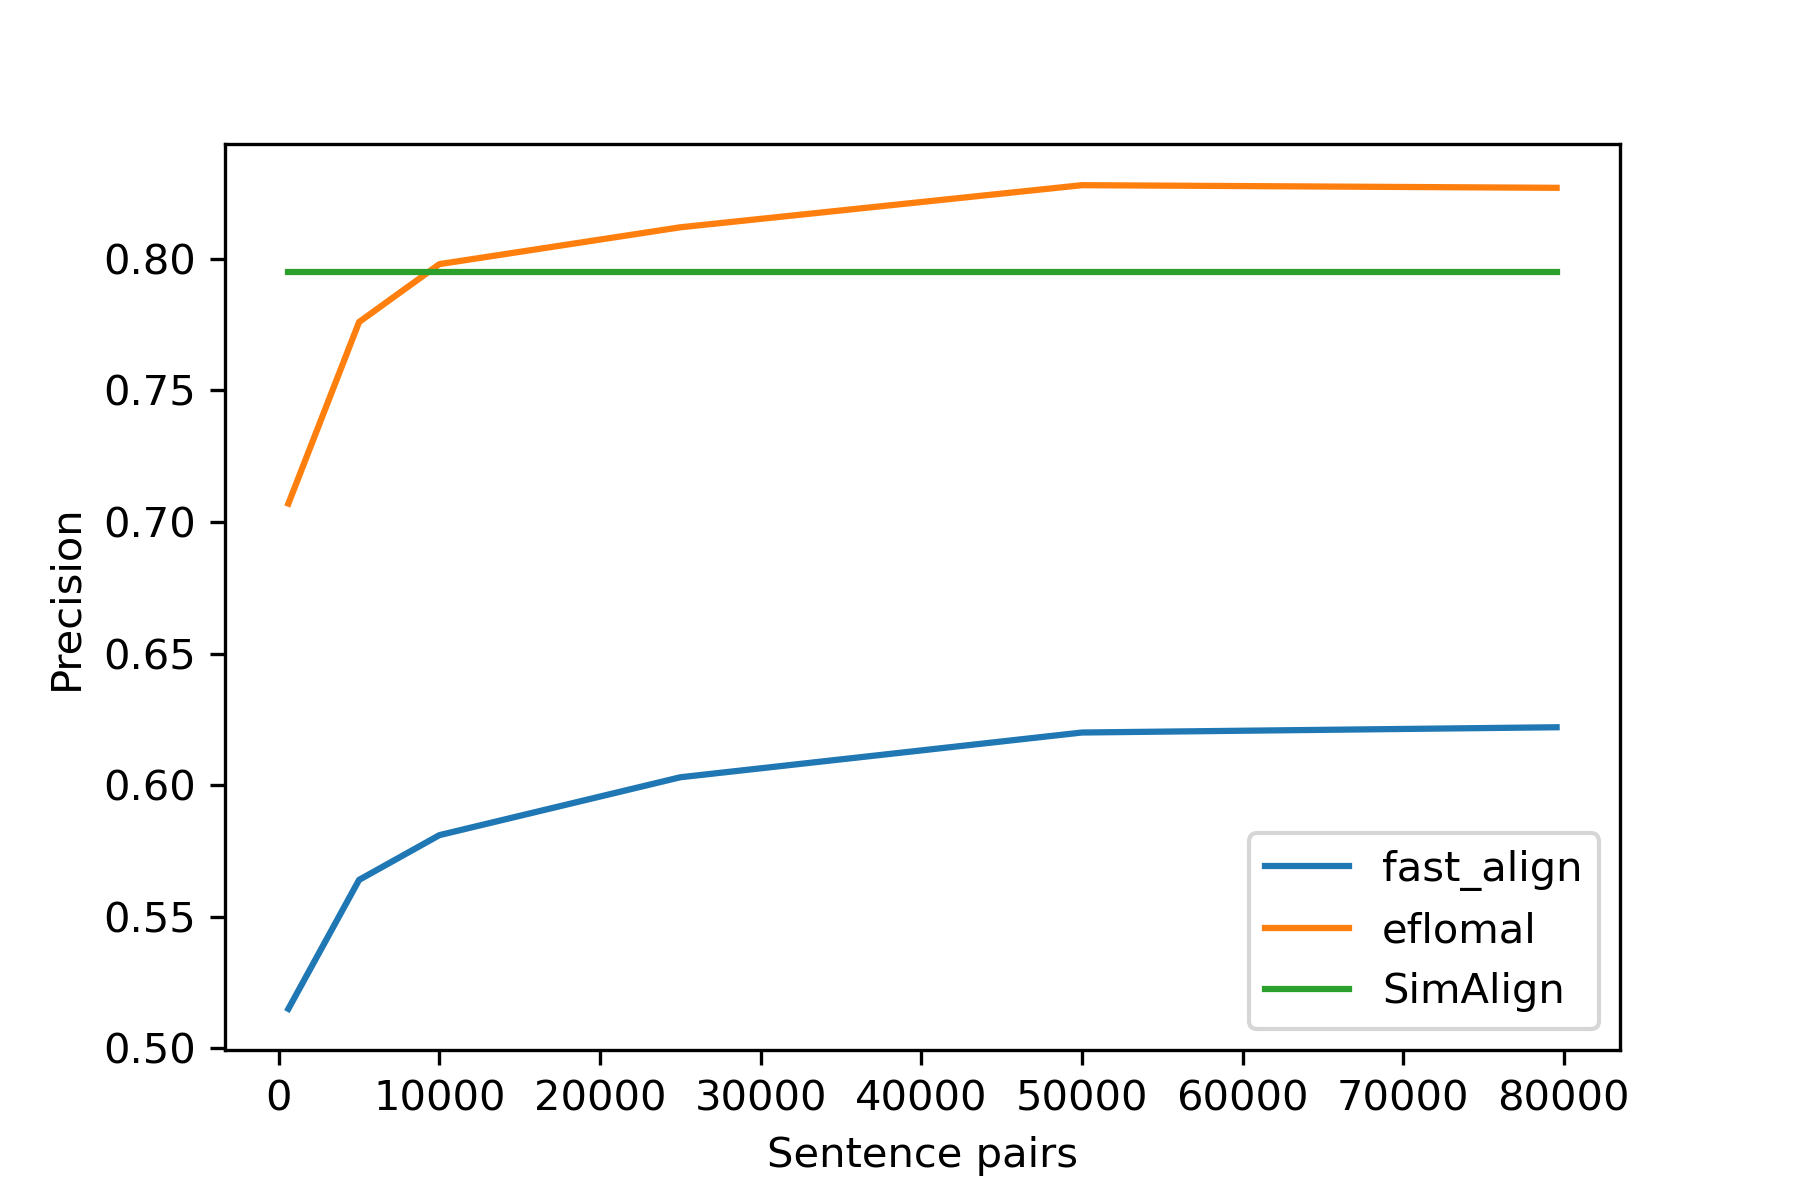
\includegraphics{graphics/charts/precision.png}
\caption{Comparing precision between the systems for different dataset sizes.}
\label{fig:precision}
\end{figure}
\begin{figure}
\centering
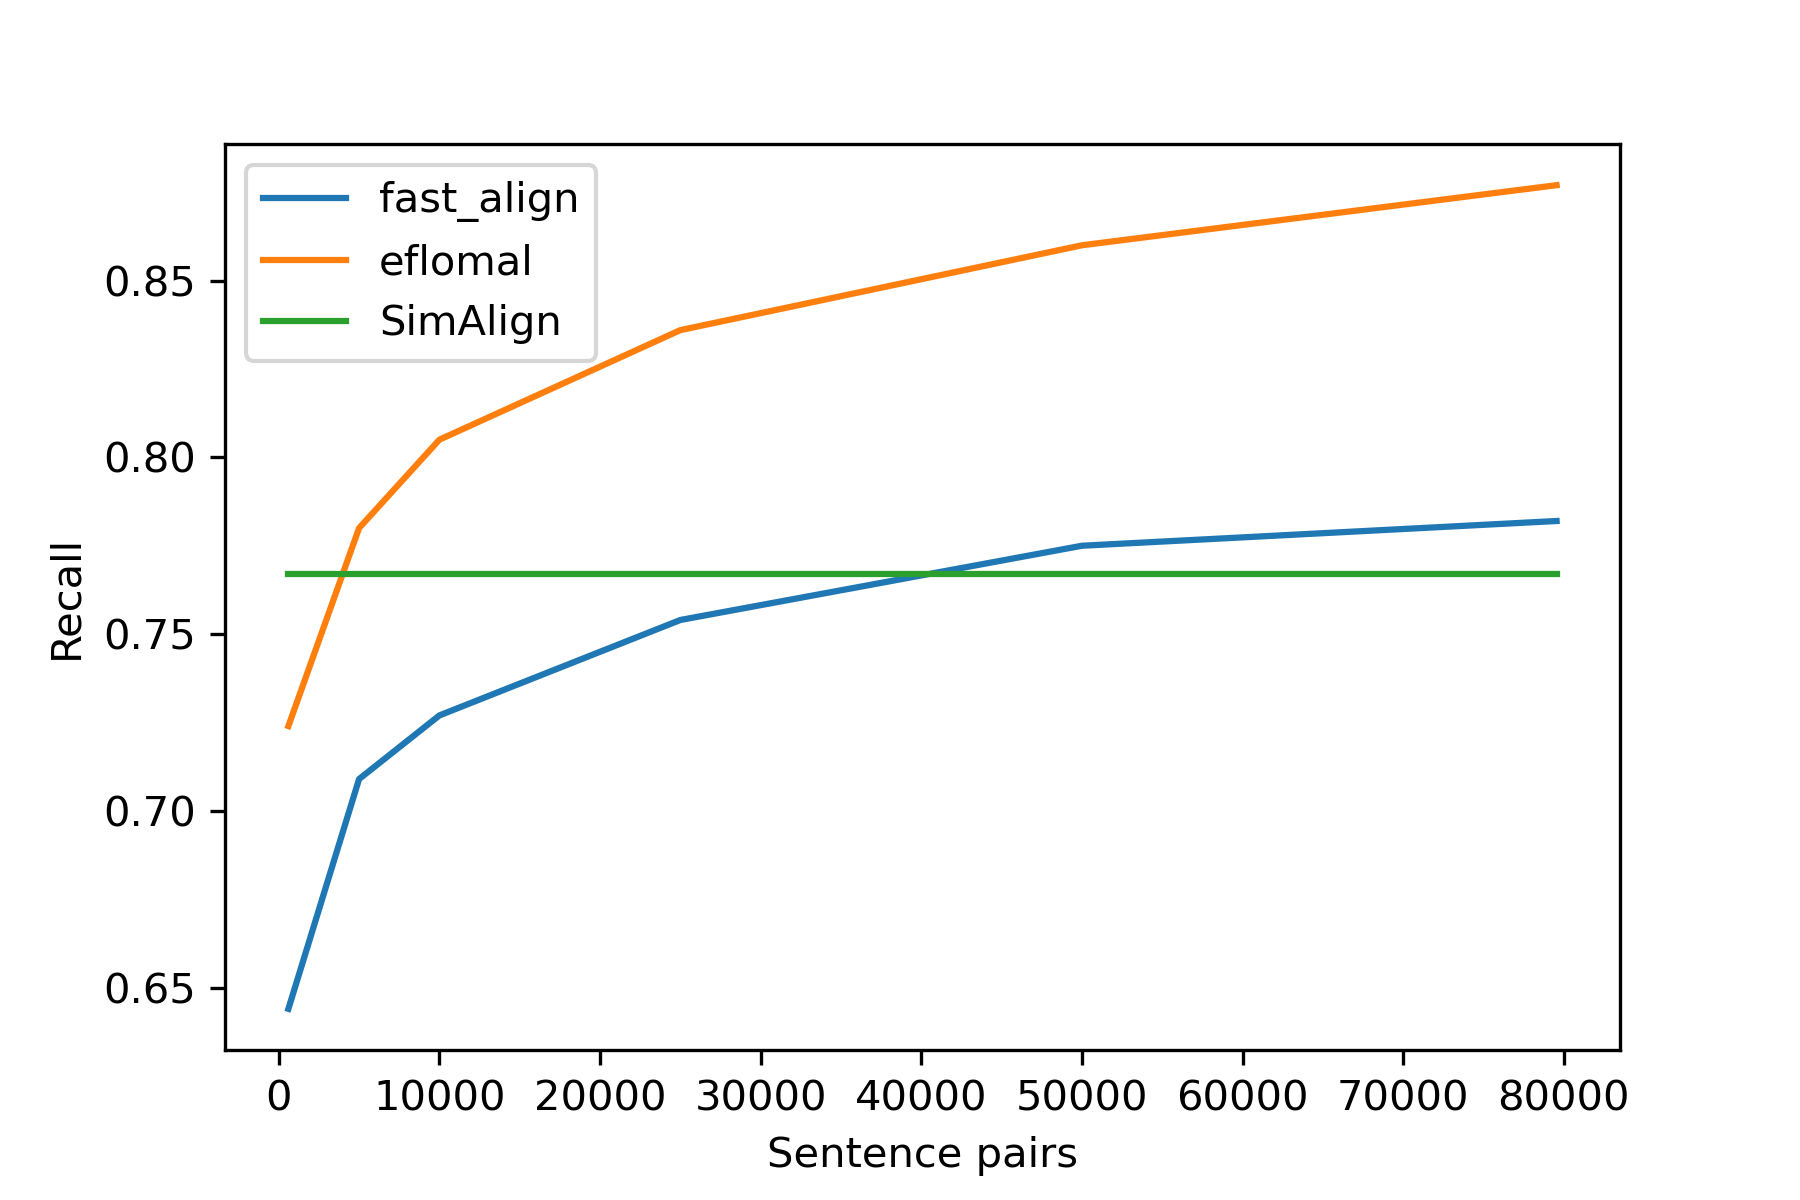
\includegraphics{graphics/charts/recall.png}
\caption{Comparing recall between the systems for different dataset sizes.}
\label{fig:recall}
\end{figure}

\begin{figure}
\centering
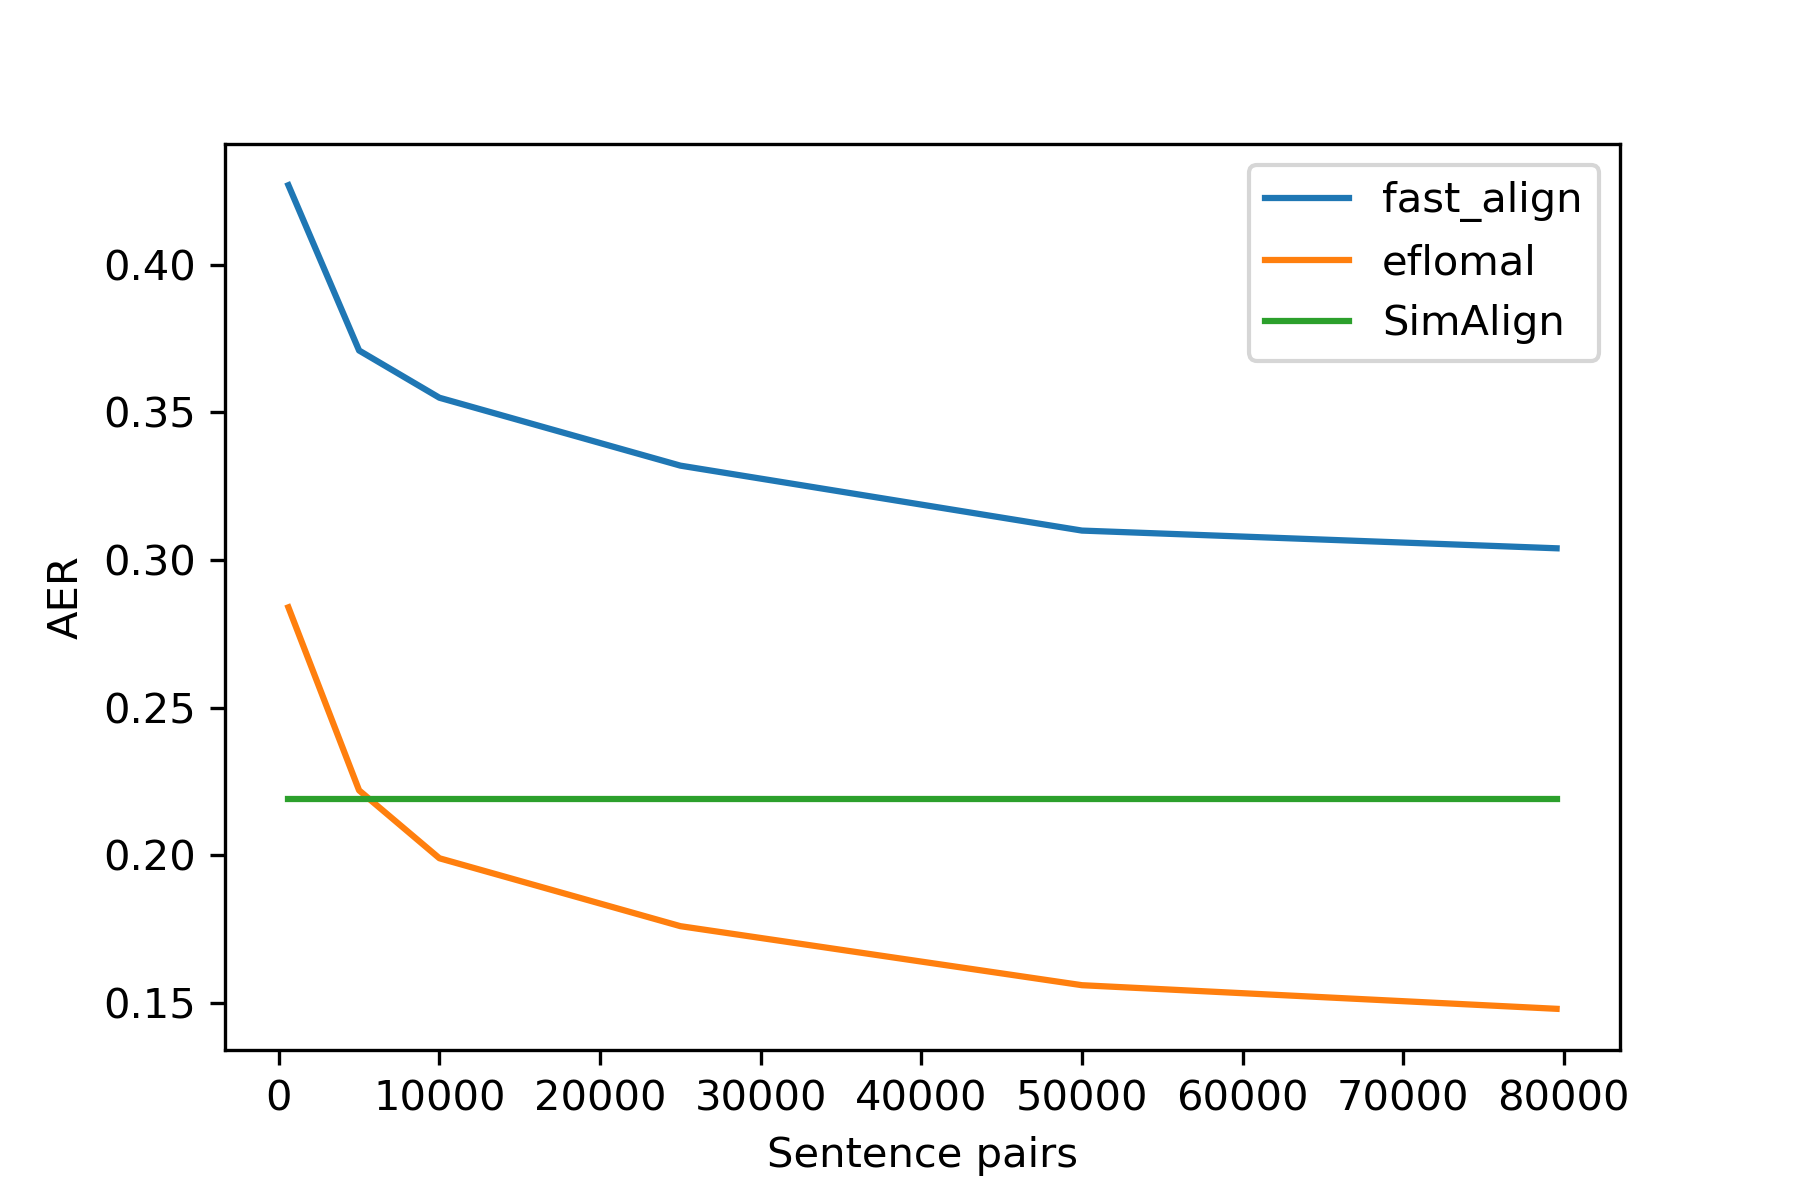
\includegraphics{graphics/charts/aer.png}
\caption{Comparing \acrshort{aer} between the systems for different dataset sizes.}
\label{fig:aer}
\end{figure}

\subsection{General Problems with Evaluation}
\label{sec:problems-evaluation}
It should also be mentioned that each word alignment gold standard has different annotation guidelines and might be more preferable or biased towards one model or the other. 
For instance a gold standard which prefers 1-to-1 alignments will reward a model which generates little or no 1-to-many alignments. 
At the same time, it will penalize the precision performance of a model that generates 1-to-many alignments, although they might be correct.

Handling Sure and Possible alignments in a different way in each gold standard might also affect the performance evaluation. 
Not using Possible alignments will lead to a lower precision value, since it will have lower values for the union of the generated alignments and the possible alignments $|A \cap P|$ (the nominator of the precision measure, see Section~\ref{sec:evaluation-metrics}). This will negatively affect precision and will penalize a model that performs better than expected. 
Labeling many of the alignments as Possible alignments instead of Sure will keep $|S|$ (the denominator of the recall measure) small and thus lead to favorable recall. 


\subsubsection{Problems with the Gold Standard for German-Romansh}
As already explained in Section~\ref{sec:gold-flaws}, the gold standard I created is not perfect (no second annotator, no Possible alignments). 
In my annotation guidelines, I preferred 1-to-1 alignments (see Section~\ref{sec:gold-principles}) and used no Possible label for labeling alignments that might still be correct.
Theoretically, not using Possible alignments may explain fast\_align's low precision. 
In theory, it is possible that fast\_align generates \emph{correct} 1-to-many alignments which I ignored in my annotations. 
In that case, we should solely concentrate on recall, which is not affected by Possible alignments. 
If we were indeed to ignore the other measurements, the difference between fast\_align (recall 0.782) and SimAlign (recall 0.767) would be 0.015 points, a difference of 2\%.

All that being said, I believe the excellent performance of eflomal proves that the gold standard is of good quality and is sensible for measuring the performance of word alignment models on German-Romansh.
 
\section{Summary}
I evaluated the performance of the two statistical baseline models (fast\_align and eflomal)  against the performance of SimAlign, a similarity based word alignment model, using a gold standard of 600 annotated sentence pairs in German-Romansh, which I had created myself.
I compared the performance of two baseline statistical models with the performance of SimAlign using multilingual embeddings in a zero-shot setting. 
SimAlign outperformed fast\_align, but not eflomal (see Table~\ref{tab:comparison}). 

SimAlign's performance, although worse the eflomal's performance, is on par with that of fast\_align and is generally promising. 
It shows that mBERT's embeddings can be used in a zero-shot setting (Romansh was not part of the training data; mBERT has never seen Romansh before) for the task of word alignment and may give future students and/or researchers the impulse to test the performance of mBERT (or other multilingual models) on Romansh in other tasks, such as information extraction, question answering, sentiment analysis etc.

See Appendix~\ref{appendix-a} for some alignment examples.



